
\begin{dialog}{…蚂蚁赋格}\label{dialog:ant-fugue}

\begin{quote}
……然后,那首赋格曲的四个声部一个接一个地插进来。
\end{quote}

\begin{dialogue}

\item[阿基里斯]我知道你们大家肯定不会相信:这个问题的答案其实近在眼前,就藏在这张图里。全部答案就是一个字——但是个无比重要的字:“无”!

\item[螃蟹]我知道你们大家肯定不会相信:这个问题的答案其实近在眼前,就藏在这张图里。全部答案就是一个词——但是个无比重要的词:“整体论”!

\item[阿基里斯]你只消盯着它瞧上一会儿,就一定能看出来。这简直同青天白日一样清楚,这张图的意思是“无”,不是“整体论”!

\item[螃蟹]对不起,我的眼睛可不是一般地好。请再看一看,然后告诉我这张图是不是有我认为它有的那种意思!

\item[食蚁兽]我知道你们大家肯定不会相信:这个问题的答案其实近在眼前,就藏在这张图里。全部答案就是一个词——但是个无比重要的词:“简化论”!

\item[螃蟹]你只消盯着它瞧上一会儿,就一定能看出来。这简直同青天白日一样清楚,这张图的意思是“整体论”,不是“简化论”!

\item[阿基里斯]又一个上当受骗的!不是什么“整体论”,也不是什么“简化论”,“无”才是这张图的意思,这再清楚不过了。

\item[食蚁兽]对不起,我的眼睛可不是一般地棒。请再看一看,然后告诉我这张图是不是有我认为它有的那种意思!

\item[阿基里斯]你们没看出来吗?上面的图案是由四条杠杠组成的,每一条杠杠都是汉字的一个笔划。

\item[螃蟹]它是由四条杠杠组成的,这点你说对了,可这些杠杠是怎么回事你却没搞对。那两条横着的杠杠分别是由两个同样的词“整体论”组成的,那条斜的和那条弯的杠杠也是由许许多多的这个词组成的,只是字要小些。这两部分的字为什么大小不一样,我不清楚,但我知道我所看到的是“整体论”,这跟青天白日一样清楚。我不明白除此之外你怎么还能看出些别的东西来。

\item[食蚁兽]它是由四条杠杠组成的,这点你说对了,可这些杠杠是怎么回事你却没搞对。那两条横着的杠杠分别是由许许多多个同样的词“简化论”组成的,那条斜的和那条弯的杠杠也分别是由三个这个词组成的,只是字要大些。这两部分的字为什么大小不一样,我不清楚,但我知道我所看到的是“简化论”,这跟青天白日一样清楚。我不明白除此之外你怎么还能看出些别的东西来。

\item[阿基里斯]我现在知道是怎么回事了。你们二位各自看到的那两个词,要么是对方看到的那个词的构成成份,要么是由对方看到的词所组成。那两条横着的杠杠确实是两个“整体论”,可这两个词全都是由用更小的字写成的许许多多个“简化论”组成的。而那两条或斜或弯的杠杠,呈一种互补的形式,则是三个“简化论”,而这三个“简化论”全是由用更小的字写成的许许多多个“整体论”组成的。这一下问题就解决了,而你们俩刚才那通愚蠢的争吵,全都是只见树木不见森林。你们明白了吗?要想正确理解这张图,就得超越“是‘整体论’还是‘简化论’”这一问题,这张画的意思应该是“无”,像你们俩这样在刚才那个问题上争来争去是毫无益处的。

\item[螃蟹]你所讲的这张图的构成我现在也看出来了,阿基,不过你说的什么“超越”之类的话,我一点也不明白。

\begin{figure}

\includegraphics{img_060.png}
\caption[“无之图”]
  {刘友庄绘。}
\end{figure}

\item[食蚁兽]你所讲的这张图的构成我现在也看出来了,阿基,不过你说的什么“无”之类的话,我一点也不明白。

\item[阿基里斯]要是你们愿意先答应我一个要求,告诉我“整体论”、“简化论”这些怪词儿都是什么意思,我就给你们解释我刚才的话。

\item[螃蟹]整体论是你能在这个世界里找得到的最普通不过的事。它是说“整体大于各个部分的总合。”只要是精神正常的人就不会反对整体论。

\item[食蚁兽]简化论是你能在这个世界里找得到的最普通不过的事。它是说“如果你理解了一个整体的各个部分,以及把这些部分‘整和’起来的机制,那么你就能够理解这个整体。”只要是精神正常的人就不会反对简化论。

\item[螃蟹]我就反对简化论。我要你给我讲讲,比方说,如何用简化论的原理来理解大脑。任何对大脑的简化论解释都不可避免地在说明“大脑所具有的意识究竟从何而来”这一问题时显得无能为力。

\item[食蚁兽]我就反对整体论。我要你给我讲讲,比方说,对蚁群的整体论描述如何比对该蚁群内蚂蚁的分别描述、它们各自的角色,以及相互间的关系等,更能说明事情的本来面目。任何对蚁群的整体论解释都不可避免地在说明“蚁群所具有的意识究竟从何而来”这一问题时显得无能为力。

\item[阿基里斯]打住吧!我刚才的那番话难道是为了引起一通新的争论吗!好啦,我现在明白你们在争论什么了,我看我对“无”的解释一定会对你们有很大的帮助。你们知道,“无”是古代禅宗对某些问题的回答,用来废问这个问题。我们现在的问题似乎是:“世界应以整体论原理来理解还是应以简化论原理来理解?”“无”这一答案把这一问题的前提,即“二者必居其一”这一规定给否定了。通过废问这个问题,揭示出更广泛的真理:存在着某种更大的领域,使得整体论与简化论的解释都适合。

\item[食蚁兽]荒谬绝伦!你这个“无”跟火车的“呜呜”声一样无聊。我不要听禅宗的什么胡言乱语。

\item[螃蟹]荒唐透顶!你这个“无”跟轮船的“呜呜”声一样无聊。我不要听禅宗的什么乱语胡言。

\item[阿基里斯]哦,天哪!我们现在谁也说不服谁。你为什么一直这么奇怪地保持沉默,龟兄?这叫我很不自在。你肯定能帮我们解脱这种困境,是吧?

\item[乌龟]我知道你们大家肯定不会相信:这个问题的答案其实近在眼前,就藏在这张图里。全部答案就是一个字——但是个无比重要的字:“无”!

\dnote{(就在他说这话的时候,那首赋格曲的第四个声部也加入进来了,正好比第一声部低一个八度。)}

\item[阿基里斯]噢,龟兄,这次你可叫我失望了。我刚才还以为像你这样一位事事都比我看得透的人,准能解决这个窘人的难题呢——可很明显,你并不比我看的更远。也好,我想我应该为这次能跟龟兄看的一样远而高兴才是。

\item[乌龟]对不起,我的眼睛可不是一般地尖。请再看一看,然后告诉我这张图是不是有我认为它有的那种意思。

\item[阿基里斯]当然有!你只不过重复了我的发现。

\item[乌龟]也许在这张图中,“无”所在的地方比你所想象的层次要低,阿基——低一个八度(形象点说)。不过我看我们可以把这个争论抽象化。我想听听阐述得更清楚些的整体论和简化论的观点,然后我们才会有根据下判断。比方说,我很愿意听一听对蚁群的简化论描述。

\item[螃蟹]也许食蚁兽大夫能告诉你一些他这方面的经验。他毕竟是这一领域里的专家。

\item[乌龟]我确信我们有很多东西要向您请教,食大夫。您能从简化论的角度对我们谈谈有关蚁群方面的事吗?

\item[食蚁兽]愿意效劳。正像老蟹对您说过的那样,我的职业使我对蚁群有着比较深入的了解。

\item[阿基里斯]可以想象!食蚁兽这一职业看来同作一名蚁群专家是一回事!

\item[食蚁兽]对不起。“食蚁兽”不是我的职业,而是我的种属。我的职业是蚁群外科医生。我的专长是用外科切除手术来治疗蚁群的神经错乱。

\item[阿基里斯]噢,是这样。可你所说的蚁群的“神经错乱”是什么意思?

\item[食蚁兽]我的大多数病人患的都是失语症。你知道,一群群的蚂蚁不得不每天乱找些词语来应付各种出现的场合,这确实是个悲剧。我是想改善这一状况,办法是,唔——清除——蚁群中出毛病的部分。这种手术有时相当复杂,要想做这种手术需要预先几年的研究功夫。

\item[阿基里斯]但是——那些患者在患失语症之前是具备语言能力的吗?

\item[食蚁兽]对。

\item[阿基里斯]可蚁群本来是不具备这种能力的,所以我有点糊涂。

\item[螃蟹]上周你没在这儿真是太糟糕了,阿基,那次食大夫和马姨到我这里来作客,我真应该把你邀来。

\item[阿基里斯]马姨是你的亲姨吗,老蟹?

\item[螃蟹]哦,不,其实她谁的姨也不是。

\item[食蚁兽]但是那可怜虫一定要每个人都叫她马姨,即使陌生人也得这样。这是她那些可爱的怪癖中的一个。

\item[螃蟹]是这样,马姨是个很怪的人,不过她可真是个活宝。上周我没有邀你过来见见她,真是太可惜了。

\item[食蚁兽]她确实是我有幸结识的蚁群中受教育最好的一个。我们俩一连好几个晚上就十分广泛的问题进行了长时间的交谈。

\item[阿基里斯]我过去一直以为食蚁兽是蚂蚁的克星,而不是蚁中知识分子的保护神。

\item[食蚁兽]啊,当然,这两者是很不一致的。我跟蚁群保持着非常良好的关系。我吃的是蚂蚁,而不是蚁群——这样做对于我和蚁群双方都是不勉为其难的。

\item[阿基里斯]怎么可能——

\item[乌龟]怎么可能——

\item[阿基里斯]——吃掉蚁群中的蚂蚁却又造福于这个蚁群?

\item[螃蟹]怎么可能——

\item[乌龟]——火烧森林却又造福于这片森林?

\item[食蚁兽]怎么可能——

\item[螃蟹]——砍掉树枝却又造福于这棵大树?

\item[食蚁兽]——给阿基里斯剃头却又造福于他?

\item[乌龟]也许你们大家讨论得太专心了,巴赫这首赋格曲里刚出现的那个漂亮的提前进入你们谁都没有注意到。

\item[阿基里斯]什么是提前进入?

\item[乌龟]哦,抱歉得很,我还以为你知道这个词呢。这个术语的意思是同一个主题在不同的声部中一次又一次地重复插入,这些插入彼此间的时间间隔非常短。

\item[阿基里斯]要是我听的赋格足够多的话,我很快就会弄懂这一切,无需别人的提示,我自己就能把它们指出来。

\item[乌龟]请原谅,朋友们。很抱歉把你们的讨论打断了。刚才食大夫正要说明吃蚂蚁是怎样同作蚁群的朋友这件事完美无缺地协调起来的。

\item[阿基里斯]嗯,我现在模模糊糊地有点明白了,有规律地吞吃些数量有限的蚂蚁会改善整个蚁群的健康状况,这事也许是可能的——可真正叫人糊涂的是跟蚁群交谈这种鬼话。这是不可能的。蚁群只是一伙单个儿的蚂蚁,只会没头没脑地跑来跑去,忙着觅食做窝什么的。

\item[食蚁兽]如果你固执地只见树木不见森林,那你可以这么说,阿基。实际上,蚁群被当作一个整体来看时,是些良定义的单位,具有自己的特点,有时这种特点还包括对语言的掌握。

\item[阿基里斯]我觉得很难想象我一个人在森林中间大喊几声,随后就能从蚁群那儿听到什么回答。

\item[食蚁兽]不开窍儿的家伙!蚁群可不是这样运用语言的。它们不是大声说出来,而是写下来。你知不知道众多的蚂蚁是如何排成一串东游西串的?

\item[阿基里斯]哦,知道——常常是直冲着我那应有尽有的厨房杀奔过去,一头钻进我的桃子酱里。

\item[食蚁兽]其实,这种串有的就用编码的形式包含着信息。要是你懂得那个系统,你就可以像读一本书一样读懂它们说了些什么。

\item[阿基里斯]了不起。你能把你的意思再反传给它们吗?

\item[食蚁兽]没问题。我跟马姨就是用这种方式交谈了数小时之久的。我拿着一根棍往湿地上画道道儿,然后看着蚂蚁们弄明白我的这些道道儿。不一会儿,有的地方开始组合成新的列串。我非常喜欢看这些列串的形成过程。在它们组合时,我就预测它们下一步会怎么办(不过我猜错的时候比猜对的时候要多)。当串的排列完成时,我就知道了马姨在想些什么,接着就该由我作出回答了。

\item[阿基里斯]这个蚁群中一定有一些聪明过人的蚂蚁,我敢肯定。

\item[食蚁兽]我看你依然没有弄明白这里面的层次区别。就像你不会把一棵树错当成一片森林一样,你在这里也不应该把一只蚂蚁当作整个蚁群。你明白吗,马姨中的所有蚂蚁要多笨就有多笨,打死它们也不会说话!

\item[阿基里斯]那么,进行交流的能力从何而来?一定是存在蚁群里的某个地方!我不明白既然马姨能一连几个小时跟你大谈特谈,妙语连珠,那些蚂蚁怎么会全都蠢笨不堪呢?

\item[乌龟]在我看来,这种情况跟由神经元组成的人脑的构成没什么不同。当然没有人会认为单个的脑细胞本身是有智能的,并用它来解释人为什么能进行有智慧的谈话。

\item[阿基里斯]哦,当然不会。关于脑细胞的问题,我完全明白你的意思。只是……风马蚁不相及呀。我是说,蚂蚁到处逛来逛去,完全是随意的,无非是时不时地弄点食物的残渣……它们想干什么就干什么,在这种随心所欲里面,我一点也看不出它们的行为作为一个整体,能体现出什么有条有理的东西来——特别是那种为交谈所必需的大脑行为中所具有的条理。

\item[螃蟹]在我看来,蚂蚁的这种随心所欲是局限在一定的范围之内的。比方说,它们可以随意游逛,互相擦拂,捡起小东西,排列成串,等等。但是它们从没有从这个小世界中,这个它们所在的蚂蚁系统中,跨出过一步。它们永远也不会这么做,因为它们没有作这种想象的智力。所以蚂蚁是种非常可靠的工具,在这种意义上说,你可以依靠它们用某种方法来从事某项任务。

\item[阿基里斯]不过,即使如此,它们在其限度之内也还是自由的,它们只是随随便便地转来转去,毫无条理,一点也不考虑作为更高一层存在的思想机能,可食大夫却宣称这些蚂蚁都只是这种更高一层存在的组成部分。

\item[食蚁兽]嗯,不过还有一点你没能看出来,阿基——统计学中的合规律性。

\item[阿基里斯]这是什么?

\item[食蚁兽]比方说,作为个体来看,即使每个蚂蚁的活动路线似乎是很随意的,然而就大量的蚂蚁来说,从这种乱糟糟的状态中,还是能看出存在着一些总的趋向。

\item[阿基里斯]哦,你的意思我明白了。事实上,蚂蚁组串是这种现象的一个极好的例子。一方面,任何一只单个蚂蚁的活动你都是无法预知的,而另一方面,串本身似乎仍然是界说良好的、稳定的。这当然意味着单个蚂蚁并不是完全随意地跑来跑去。

\item[食蚁兽]完全正确,阿基。蚂蚁之间存在着某种程度的交流,这种信息传递恰好足以使它们避免完全随意的活动。靠着这种最低限度的交流。蚂蚁们可以互相提醒,以使它们意识到它们不是孤单的,而是正在同队友进行合作。这样就能调集大量的蚂蚁,用这种方式互相支援,去从事随便什么活动——例如组串——只是所需时间不限。我对脑外科手术模模糊糊的认识使得我坚信神经元的发射情形也是这样。一大堆神经元发射脉冲,以使另一个神经元发射,不是这样吗,老蟹?

\item[螃蟹]肯定是这样。以阿基里斯大脑中的神经元为例吧。每个神经元都从与它的输入线连在一起的那些神经元接收信号,如果输入的总和在某一时刻超过了临界点,这个神经元就会发射,并把它自己的输出脉冲传递到别的神经元,而这后一神经元也将发射——并沿着这条线一直传送下去。神经讯号沿着阿基里斯的路径毫不延迟地迅猛掠过,那架势比飞燕俯冲捕食蚊蚋还有过之无不及。每段曲折、每个回转,都由阿基里斯大脑中的神经结构预先排定,直至输入感觉的讯号产生了影响。

\item[阿基里斯]在正常情况下,我觉得我想些什么是受我自己控制的——可按你这种说法就整个儿颠倒了,你的意思好像是说“我”只是所有这些神经结构、自然规律控制的某种有机体的副产品,往坏里说则是由我那被歪曲了的感觉所造成的某种人为概念。换句话说,你让我觉得我并不知道我是谁——或者是什么——如果我还是个什么的话。

\item[乌龟]随着我们讨论的继续,你会越来越明白的。但是,食大夫——你用这种类比来说明什么呢?

\item[食蚁兽]我以前就注意到,在这两个彼此非常不同的系统中存在着某种相一致的东西。现在,我对这一点的认识更进一步了。事情似乎是——以排列成串为例来说——只有当蚂蚁的数量达到某一临界数量时,有条理的蚁群现象才会出现。如果出现了某种指向某一目标的活动,这也许是某一地带少数蚂蚁的行为,那么就会发生下面两种情况中的一种:或者是在一个短暂而热闹的开头之后夭折——

\item[阿基里斯]因为没有足够多的蚂蚁把这一活动进行下去?

\item[食蚁兽]一点不错。另一种情况是蚂蚁的数量达到了临界指标,那样一来那项活动就会像滚雪球一样,把越来越多的蚂蚁裹挟进来。在这后一种情况下,一个为同一目标而工作的完整的“蚁队”就出现了。这一目标可能是要排成串,或是为了收集食物,或许还可能是为了造窝。尽管这种结构规模很小,又十分简单,可它会在更大的规模上产生十分复杂的后果。

\item[阿基里斯]我现在已经能从你的描述里掌握“紊乱中的有序”这个观念了,可这离具有交谈能力还差得远呢。气体分子的随意碰撞同样也是混乱中的有序——这种混乱有三种参数可以对它进行描述:这就是体积、压强和温度。这同具有理解世界或谈论世界的能力的要求,还差得远呢!

\item[食蚁兽]这显示出在对蚁群行为的解释与对某一容器中气体行为的解释之间,存在着某种非常有趣的区别。解释气体的行为只要计算一下其分子运动的统计规律就行了。除了考虑这种气体本身以外,无需讨论别的什么比分子更高一层的结构因素。而在另一种情况下,对于蚁群,除非你弄清了结构的各个层次,否则你便无法理解——哪怕一点儿——这个蚁群的活动。

\item[阿基里斯]你的意思我明白了。在气体的研究里,你可以从最低的层次——分子——一下子跳到最高的层次——气体本身。不存在结构上的中间层次。那么,蚁群中是怎样产生作为中间层次的有条理活动的呢?

\item[食蚁兽]这跟蚁群内存在着好几种不同种类别的蚂蚁有关。

\item[阿基里斯]哦,对。我想我听说过这一点。这种现象被称作“种姓制”,对吗?

\item[食蚁兽]完全正确。除了蚁王,还有雄蚁,事实上,养家糊口的事它们是不管的,此外还有——

\item[阿基里斯]当然还有战士——光荣的反共战士!

\item[螃蟹]嗯……这恐怕不对,阿基。蚁群的内部是很共产主义化的,那它们的战士干嘛要反共?我说的对吗,食大夫?

\item[食蚁兽]是的,你对蚁群的说法是对的,老蟹,它们确实建立在某种共产主义的原则上。至于那些战士,阿基想得有点天真。其实,这些所谓“战士”几乎根本不会打仗。它们是些长着大脑袋的行动迟缓、动作笨拙的家伙,它们长着一副利颌,用来啃咬东西,不过它们可谈不上什么“光荣的”。正像在真正的共产主义社会里那样,工蚁才被称作是光荣的。大多数的家务都是由它们来做的,比如觅食、巡猎、带幼虫等。大多数的战争也是由它们去打的。

\item[阿基里斯]嗬。这事真荒唐。战士不打仗!

\item[食蚁兽]嗯,我刚说过的,它们根本不是什么战士。工蚁才是真正的战士,而那些所谓的战士——其实应该叫兵蚁——都是些又懒又呆的家伙。

\item[阿基里斯]哦,太可耻了!哼,我要是只蚂蚁,一定给它们规定些纪律!让那些呆脑壳开开窍儿!

\item[乌龟]你要是只蚂蚁!你怎么会是只蚂蚁!根本没法把你的大脑映射成蚂蚁的大脑,我看在这个问题上绞尽脑汁是不会有什么结果的。把你的大脑映射到蚁群中才是个更合理的命题……不过我们先别把话题岔开。让食大夫继续对蚂蚁组织中更高层次的种姓制和它们的角色做精彩的描述吧。

\item[食蚁兽]好吧。一个蚁群中有各式各样的任务需要完成,而单个的蚂蚁则发展了各种专长。蚂蚁的专长通常随蚂蚁年龄的变化而变化。当然,这也依赖于它们所在的种姓。任何一时刻的任何一个蚁群里,所有类别的蚂蚁都同时存在。在某些地方也许某种种姓的蚂蚁很稀少,而在别的地方也许很稠密。

\item[螃蟹]某一特定种姓或专长的蚂蚁,其稠密度是随意的吗?或者换句话说,在某一地区某一类的蚂蚁分布得很集中,在另一地区不那么集中,是有什么原因的吗?

\item[食蚁兽]你这个问题提得很好,这对理解蚁群是如何思想的有着至关重要的意义。实际上,一个蚁群内各种姓的分布是很严格的,是长期进化的结果。正是这种分布规律使蚁群达到了能同我进行交谈的复杂程度。

\item[阿基里斯]在我看来,蚂蚁们来来去去的不断活动使分布的严格性完全不可能了。蚂蚁们那种随意的活动会很快地破坏掉分布的严格性,正像某种气体中分子的固定格局由于各方面分子的随意碰撞,一刻也不能存在一样。

\item[食蚁兽]在蚁群里,情况正相反。事实上,恰恰是蚁群中蚂蚁们这种来呀去呀永不停息的活动,使得种姓分布能适应不断变化的情况,因而也就保持了合适的种姓分布。你明白吗,种姓分布并不是始终如一、严格不变的,而是必须要不断变化,从而以某种方式反映出蚁群所处的现实世界的环境。正是蚁群里的这种活动使种姓分布不断得到更新,使蚁群能同所面临的现时环境相适应。

\item[乌龟]能举个例子吗?

\item[食蚁兽]当然可以。当我,一只食蚁兽,来拜访马姨时,那些呆头呆脑的蚂蚁因为闻到了我的气味,全都吓得张皇失措——当然,这就是说,它们全都从我来之前它们所在的地方四散奔逃了。

\item[阿基里斯]不过这可以理解,你是蚁群的凶敌嘛。

\item[食蚁兽]哦,不。我必须重申,我根本不是蚁群的敌人,我是马姨最对劲儿的伙伴。而马姨则是最对我口味儿的姨。说蚁群中所有单个的蚂蚁都很怕我,这我同意——可这完全是另一码事。无论如何,你能理解了吧:由于我的到来所引起的蚂蚁的活动,完全改变了蚂蚁的内部分布。

\item[阿基里斯]很明白了。

\item[食蚁兽]这就是我刚才说过的更新。新的分布反映出了我的存在。这种从过去的状态向新状态的改变,可以被说成是使蚁群增添了“一条知识”。

\item[阿基里斯]你怎么能把一个蚁群内不同类型蚂蚁的分布说成是“一条知识”?

\item[食蚁兽]这里面有个至关重要的问题,需要详细解释。你知道吗,接下来的问题是你打算如何描述种姓分布。如果你继续用低层次的单位——单个的蚂蚁——来思考问题,那你就会只见树木,不见森林。这种层次太微观了,当你从微观的角度进行思考时,你必然会漏掉更大规模上的现象。你不得不用更恰当的高层次上的构架来描述种姓分布——只有这样,种姓分布如何能编码出许多条知识这一问题才有意义。

\item[阿基里斯]那么,那种用来描述蚁群现存状态的恰当单位,你是怎么找到的?

\item[食蚁兽]好吧,让我们从最基本的说起。当蚂蚁想做成某件事时,它们就组成各种小“蚁队”,也就是凑在一起去干一件事。就像我前面提到过的那样,蚂蚁们的小团伙总是在不断地形成和解散。那些实际上能存在一段时间的就是各种蚁队,它们没有散伙的原因就是因为有事情需要它们去做。

\item[阿基里斯]可前面你说过如果一群蚂蚁的规模超过了某一临界点,这个群体就会集聚在一起。现在你又说如果有什么事可做,这个群体就会集聚在一起。

\item[食蚁兽]这两种说法意义是一样的。比方说,在觅食时,如果某个闲逛的蚂蚁在某个地方发现了一些食物,并想把这个喜讯传给别的蚂蚁们,那么,作出反应的蚂蚁数量将会同食物样品的大小相一致——太少的数量将不会吸引足以超过临界点数量的蚂蚁。这也正是我所谓的无事可做的意思——食物少得不值得去重视。

\item[阿基里斯]我明白了。我应该假定这些“蚁队”是结构中的一个层次,处在单个蚂蚁的层次和蚁群的层次之间。

\item[食蚁兽]正是这样。有一种类型特别的蚁队,我把它称作“信号”——结构中所有的更高级的层次都建立在信号上。事实上,一切比信号更高级的实体都只是由行动协调一致的信号所组成的集合。高层次上的队其组成单位不是蚂蚁,而是些低层次上的队。这样一直找下去,最后就到了最低层次的队——也就是所谓的信号——在这之下,才是蚂蚁。

\item[阿基里斯]它们为什么叫“信号”这样一个容易引起联想的名字?

\item[食蚁兽]这名字是指它们的功能。信号的作用是把具有各种专长的蚂蚁输送到蚁群中需要的部分。因此信号的典型活动是这样的:信号的产生是由于蚂蚁数量超过了维持一个信号的存在所必需的临界点,随后这个信号便通过蚁群向远处传递,在某些时候,信号便多多少少分解还原成为其单个的组成部分,并丢下它们不管。

\item[阿基里斯]听起来有点像波浪,从远处挟裹来一些海星、海草,把它们孤零零地拋到了岸上,丢下它们不管。

\item[食蚁兽]在某种意义上这种类比是对的,蚁队确实抛下了一些它从远处带来的东西,可海浪还是要回到海里的,而在信号这里,就没有类似的载体,因为信号是由蚂蚁组成的。

\item[乌龟]我觉得一个信号只是在途经该蚁群中原来需要这类蚂蚁的地方时,才会分解掉。

\item[食蚁兽]那自然。

\item[阿基里斯]那自然?在我看来,某个信号总能到达原来需要它的那个地方这种事,并非那么显而易见。即使它传播的方向正确,它怎么能判断出它应该在哪儿解散?它怎么知道它已经到了该去的地方了?

\item[食蚁兽]这是个极端重要的问题,因为这涉及到对有目的的行为——或者说是似乎有目的的行为——从信号角度所作的解释。从对它们的描述里,人们倾向于把信号的行为说成是旨在满足需要,从而把它称作“有目的”的。但你也可以从别的角度看这一问题。

\item[阿基里斯]哎,等等。要么这种行为是有目的的,要么不是。我不明白怎么能又是又不是。

\item[食蚁兽]我来给你解释一下我看问题的方式,看你是否同意。一个信号一旦形成,这个信号本身并不考虑它应该往哪个方向传播。在这里起决定作用的是种姓分布。是它决定着信号在蚁群中的运动,以及这个信号能持续多长时间、在哪里“解散”。

\item[阿基里斯]这么说一切都依赖于种姓分布,是吗?

\item[食蚁兽]正是这样。让我先来描述一下正在传播中的一个信号。当信号发出的时候,组成这一信号的蚂蚁们或是通过直接的接触,或是依靠气味的传达,同位置上与它们相邻的蚂蚁进行合作,以使信号通过。这种接触与气味报道了某个地方出现了需求,诸如筑窝、哺育等这类事情。只要这种局部的要求还得不到满足,这个信号就会一直保持下去。但是一旦出现一批蚂蚁能够满足那一需求,信号便会解散,而奔赴来救急的蚁队就在现场全面铺开,进行工作。现在,你明白蚁群中的种姓分布如何发挥各队的指导作用是怎么回事了吗?

\item[阿基里斯]很明白了。

\item[食蚁兽]这种观察事物的方法并不要给这种信号加上个什么目的,这一点你也明白了吧?

\item[阿基里斯]是的。的确,我开始学会从两种互不相同的角度来看这一问题了。从蚂蚁的眼睛所看到的角度,信号是无目的的。信号中普通的蚂蚁只是在蚁群附近逛来逛去,没有什么特定的目的,直到发现了什么它觉得还可以的东西后,才停下来。它的队友们常常也同它意见一致,于是这时蚁队才算完成了任务,原地解散,有组织的集合就不复存在了,而只剩下一些散兵游勇。没有什么计划啦、事先的预测啦这一类东西,也不需要什么侦察来决定正确的方向。然而从蚁群的角度看,蚁队的行为却是对以种姓分布这种语言写成的信息所作的反应。所以从这一角度看,这种行为显得很像是有一定的目的。

\item[螃蟹]如果种姓分布完全是随意的,那会怎么样?那些信号还会结聚和解散吗?

\item[食蚁兽]当然啦。不过这个蚁群将不会保持多久,这是因为它的种姓分布是无意义的。

\item[螃蟹]这正是我想弄明白的。蚁群的存在是由于它的种姓分布有一定的意义,而这一意义是在其整体水平上产生的。在比整体水平低的层次上,是看不到这种意义的。你除非在这种高层次上进行解释,否则就无法读懂它的意思。

\item[食蚁兽]我明白你的观点,不过我看你把问题想得太狭隘了。

\item[螃蟹]怎么?

\item[食蚁兽]蚁群几十亿年来一直在经历着严酷的进化选择。只有少数一些机制被选择出来,而大部分都被淘汰了。结果就形成了我们现在正在讨论的支配着蚁群的这一套机制。如果你能在电影上观察这一完整的过程——当然,这比实际进程要快上差不多十亿倍——你就会觉得各种机制的出现完全是对外界压力的自然反应,就像开水冒泡是对外在的热源的自然反应一样。我想你不会觉得开水冒泡有什么“意义”和“目的”——不过,也许你会?

\item[螃蟹]不,但是——

\item[食蚁兽]这就是我的观点。无论泡沫有多大,其产生都可以追溯到分子水平,你可以不管什么“高层次的规律”。蚁群和蚁队的道理也是一样的。通过从进化这一开阔的角度考虑这一问题,你就可以排除有意义有目的的蚁群这一想法。这样它们就变得可有可无了。

\item[阿基里斯]哎,食大夫,你不是刚告诉我们你跟马姨交谈过吗?现在看来你要否认她能交谈或思想啦。

\item[食蚁兽]我没有自相矛盾,阿基。你知道,同别的人一样,用这么巨大的时间单位去观察事物,对我来说也是很困难的,所以我觉得改换一下角度会更方便些。当我撇开进化过程而对此时此地的现象进行观察的时候,就又回到了那种目的论式的语言:即种姓分布的意义和信号的有目的性。我不仅在考虑蚁群时采用这种角度,而且当我考虑我自己和别人的大脑时,也是如此。不过,如果必要的话,我也能采用别的角度,把意义排除于这些系统之外,只是这多少要费点劲儿。

\item[螃蟹]进化的确能创造奇迹,正像你没法儿从创造奇迹的魔术师那里预知他又要从袖子里抖落出什么东西一样,你也无法猜测进化下一次将会弄出什么玩艺儿来。比方说,要是出现这样的事,我一点儿也不会感到吃惊:如果在理论上可能,有两个或更多的“信号”彼此交错,每一个都不知道另一个也是一个信号——每一个都把另一个仅仅当作是一般状态的蚂蚁群。

\item[食蚁兽]这不仅是理论上可能的,事实中也是常有的!

\item[阿基里斯]哟……我脑子里冒出来一个什么怪念头啊。我在想象蚂蚁们朝四个不同的方向运动,有黑的,有灰的,互相交错,共同组成一个有序的图案,就像——就像——

\item[乌龟]你是说像一首赋格曲?

\item[阿基里斯]对——正是!一首蚂蚁赋格。

\item[螃蟹]很有趣的念头,阿基。不过,说到开水倒让我想起茶来了。谁想再要点儿?

\item[阿基里斯]我再要一杯,老蟹。

\item[螃蟹]行啊。

\item[阿基里斯]你认为可以把这样一首“蚂蚁赋格”分解成彼此不同的可见的“声部”,是吗?这可太难了,我是说,如果我要——

\item[乌龟]我不要,谢谢。

\item[阿基里斯]——在一首赋格曲中——

\item[食蚁兽]要是不太麻烦的话——

\begin{figure}
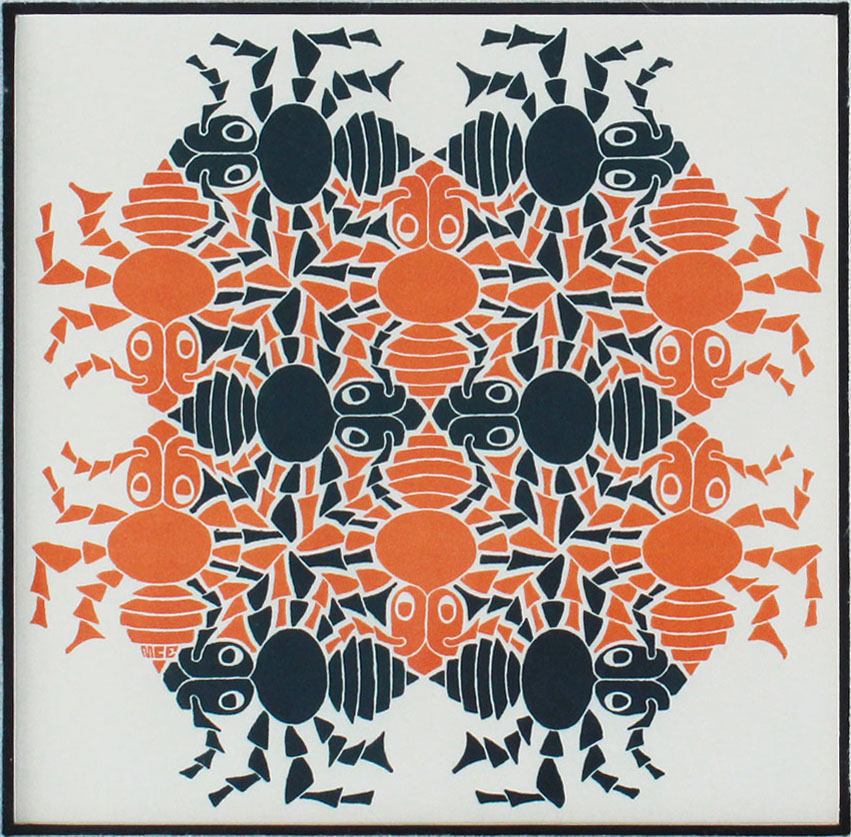
\includegraphics{img_061.jpg}
\caption[“蚂蚁赋格”,艾舍尔作。]
  {“蚂蚁赋格”,艾舍尔作(木刻,1953)。}
\end{figure}

\item[阿基里斯]——跟踪其中某一个声部——

\item[食蚁兽]——我也想来点儿,老蟹。

\item[阿基里斯]——而所有那些——

\item[螃蟹]区区小事。四杯茶——

\item[乌龟]三杯!

\item[阿基里斯]——声部都在同时进行。

\item[螃蟹]——转眼就得!

\item[食蚁兽]这个想法很有意思,阿基。不过没有人能让人信服地画出这种画来。

\item[阿基里斯]太令人遗憾了。

\item[乌龟]这个问题也许你能回答,食大夫。一个信号,从它形成到解散,总是由同样一群蚂蚁组成吗?中间不会换吗?

\item[食蚁兽]实际上,如果附近有同样种姓的蚂蚁,信号中的蚂蚁经常脱离信号而由别的同种姓的蚂蚁来替代。大多数情况下,当信号解体的时候,组成这一信号的蚂蚁已经全都不是当初形成这一信号时的蚂蚁了。

\item[螃蟹]我搞清楚是怎么一回事了:蚁群中的信号不断影响种姓分布,这一活动是对蚁群内部的要求所作出的反应,而蚁群的这种内部要求则又是蚁群对其所处外部环境的反应。因此,正如您所说的那样,食大夫,种姓的分布不断地调节、变化,最终反映着外部世界。

\item[阿基里斯]可结构中的那些中间层次是怎么回事?你刚才一直在说种姓分布最好应该以由别的蚁队组成的蚁队为单位来描述,而不应以蚂蚁或信号为单位来描述,那些组成蚁队的蚁队又是由一些别的蚁队组成的,同理下推,直至组成蚁队的成员是单个儿的蚂蚁,而不再是蚁队。你还说,要想理解种姓分布何以能被描述为某种有关外部世界的编码了的信息,这个观点是关键性的。

\item[食蚁兽]正是,我们现在正要谈这个问题。我喜欢把某些层次较高的蚁队称作“符号”。你要注意,这个词在这里的意思与它通常的意义有所不同。我所说的“符号”是指一个复杂系统的主动的子系统,这种子系统是由更低层次的主动的子系统构成的……因此,它们与被动的符号很不一样,那些被动的符号在系统之外。汉字中的笔划或单个儿的音符,都属于这种符号,它们是死的,有待于某个主动的系统去处理它们。

\item[阿基里斯]噢,这可真够复杂的。我一点儿也没想到蚁群具有如此抽象的结构。

\item[食蚁兽]是的,很了不起。不过,结构中的所有这些层次对于各种各类知识的储存都是必需的,有了这种知识储存,才能使这个机制变成“有智能的”,“有智能的”的意思在这里可以是这个词的任何合理的涵意。任何能运用语言的系统都基本上具有与此相同的一套内部层次。

\item[阿基里斯]先慢着点。你是不是暗示说我的大脑实际上也是由一群窜来窜去的蚂蚁组成的?

\item[食蚁兽]哦,不。你不要从字面意义上理解我的话。最低的层次是全然不同的。比方说,食蚁兽的大脑就不是由蚂蚁组成的。但是你如果从大脑的最低层上溯一两个层次的话,你就会发现这些层次的机制在别的具有同等智力的系统中——比如蚁群中——有与它完全一致的对应物。

\item[乌龟]这就是把你的大脑映射到蚁群中去,而不是映射到蚂蚁的大脑中去的依据,阿基。

\item[阿基里斯]对你的这份夸奖我领情了。不过这种映射是怎样进行的?比方说,我大脑中的什么东西对应于你所谓的信号这种低层次的蚁队呢?

\item[食蚁兽]哦,我对大脑的研究只是种业余爱好,所以无法一一细述它的神异之处。可是——如有不妥之处,老蟹,请不吝赐教——我猜测,在大脑中对应于蚁群里信号的那种东西是兴奋的神经元。或者,也可能是某种更大范围上的活动,比如神经元兴奋的模式什么的。

\item[螃蟹]我没有什么异议。不过你是否觉得,找出确切的对应物这一问题,即使有希望得到解决,相对于我们这场讨论的目的来说,也并不是什么十分紧要的事。在我看来,最重要的是知道确实存在着这种对应,即使我们此时此刻还不完全清楚这种对应指的是哪一部分也没有关系。我只想对你提出的问题中的一点追问一下,食大夫,因为这一问题涉及究竟在哪个层次上,人们可以断定开始产生了这种对应关系。你似乎认为一个信号在大脑中有其直接的对应部分,然而我觉得只是在你所谓的“主动的符号”这一层次上,才可能存在那种对应关系。

\item[食蚁兽]你的解释比我的更确切,老蟹。多亏你提出这个微妙的问题。

\item[阿基里斯]有什么事情只能由符号做而不能由信号做?

\item[食蚁兽]这情形有点像字与笔划之间的区别。字作为具有意义的单位,是由笔划组成的,而笔划本身却不具有意义。这也正是符号与信号的区别所在。这实际上是个很有用的类比,条件是你不要忘了字和笔划是被动的,而符号与信号却是主动的。

\item[阿基里斯]我一定会记住的,不过我不敢说我理解了为什么强调主动与被动两种性质的区别具有如此重要的意义。

\item[食蚁兽]原因在于你加于被动符号上的意义,例如一页书中的某个字,实际上来源于你大脑中与之相对应的主动符号所产生的意义。因此,只有当一个被动符号的意义与主动符号的意义发生关系时,这个被动符号的意义才能被正确理解。

\item[阿基里斯]明白了。可是究竟是什么赋予一个符号——确切地说,是主动的符号——以意义的呢?信号虽然也是一种很出色的东西,可你却说它不具有意义。

\item[食蚁兽]这与符号可以使其它符号被触发的方式有关。当某一符号成为主动时,它并非是孤立无援的。它可以通过某种媒介——在蚂蚁这里就是种姓分布——传播开来。

\item[螃蟹]当然,大脑里是没有种姓分布这类玩意儿的,在大脑中,与种姓分布相对应的是“大脑状态”。你必须描述出所有神经元的状态、所有它们交互联系的状态,以及使每个神经元触发的临界点。

\item[食蚁兽]一点不错。现在让我们把“种姓分布”和“大脑状态”都一并归于一个共同的名称之下,这个共同的名称就是“状态”。这样,这种状态就可以在某种更低或更高的层次上描述出来了。对蚁群状态进行低层次上的描述将会非常麻烦,这需要确定每个蚂蚁的位置、年龄、种姓,以及其他一些诸如此类的事情。这种详细的描述实际上无助于统观为什么该蚁群处于这种状态。另一方面,在更高层次上进行的描述则需要逐一查清哪些符号可以被哪些其他符号的组合所触发,以及触发的条件等等。

\item[阿基里斯]在信号或蚁队层次上进行的描述会怎么样呢?

\item[食蚁兽]这种描述所在的层次位于较低的层次和符号层次之间。对于在蚁群中某一特定位置上正在发生的事,这种描述能提供相当多的信息,虽然这要比一个蚂蚁一个蚂蚁的描述所含的信息少些,这是因为蚁队是由一团团的蚂蚁组成的。那种一个蚁队一个蚁队的描述就好像是一个蚂蚁一个蚂蚁描述的提要。然而,在蚁队层次上的描述必须加进一些在蚂蚁层次上所没有的内容——例如各蚁队之间的相互关系,散于各处的各种种姓的补充力量。这种新添的复杂性是你进行这种概括所必须付出的代价。

\item[阿基里斯]我觉得对不同层次上的描述进行比较是件非常有意思的事。最高层次上的描述似乎最具有解释力,在这一层描述中,你能得到关于蚁群的最直观的印象,然而,说来奇怪的是,这种描述却撇开了似乎是最重要的方面——蚂蚁。

\item[食蚁兽]不过你要明白,尽管你所看到的都不过是蚂蚁,可它们却全然不是最重要的方面。我们承认,如果没有这些蚂蚁,蚁群就不会存在。可是,与之相应的某种东西都是存在的——比如大脑——完全不依赖蚂蚁的存在而存在。因此,至少从一种高层次的观点上看,蚂蚁是可有可无的。

\item[阿基里斯]我敢说没有任何蚂蚁会热烈拥护你的这种理论。

\item[食蚁兽]不过,我从没有见过什么蚂蚁具有高层次的观点。

\item[螃蟹]你的这番描述太违背人们的直观了,食大夫。如果你所言不差,事情似乎就会是:为了了解整个儿结构,你必须省略掉构成这一结构的任何最基本的组成材料。

\item[食蚁兽]也许我打一个比方你们就能更清楚些了。请想象一下你面前摆着一本查尔斯·狄更斯的小说。

\item[阿基里斯]《匹克威克外传》——可以吗?

\item[食蚁兽]再好没有了!现在我们就来做这样一个游戏:你先想办法使每种笔划都具有意义,这样当你一个笔划一个笔划地读这本书时,整部《匹克威克外传》就都具有意义了。

\item[阿基里斯]嗯……你是说我每见到一个字,就比如“人”字吧,就要把它看作是两个各具某种一定意义的概念,并且是一个接一个地紧挨着,每种相同的笔划的意义总是一定的,没有任何变化,是吗?

\item[食蚁兽]正是这样。这样一来就只有“丿”概念、“{\CJKfontspec{MingLiU}㇏}”概念了——而且你每次碰到它们时,它们的意思都同前面它们出现时的意思一样。

\item[阿基里斯]嗬,这么一来,“阅读”《匹克威克外传》的活动简直就变成了一场难以言状的噩梦了。不管我赋予每个笔划什么意义,这一切都只不过是一场徒劳无益的玩弄无意义的游戏。

\item[食蚁兽]没错儿。单个儿的笔划与现实世界之间不存在什么自然的映射关系。只有在更高的层次上才会有这种自然的映射——即在字词与现实世界的各部分之间。你如果要叙述这本书的内容,你就不要涉及它的笔划层次。

\item[阿基里斯]当然不会!我只会叙述情节、人物这一类的东西。

\item[食蚁兽]这你就对了。你应该完全略去这本书的构成材料,即使这本书有赖于它们。它们是媒介,而不是信息。

\item[阿基里斯]明白了——那么,蚁群呢?

\item[食蚁兽]在蚁群这里,主动的信号代替了被动的笔划,主动的符号代替了被动的字词——不过原理是一样的。

\item[阿基里斯]你是说在信号与现实世界之间无法建立起映射关系?

\item[食蚁兽]你会发现你无法通过触发某个新的信号来使它具有什么意义。在比它更低的层次上——如蚂蚁层次——也同样办不到。只有在符号层次上,触发模式才有意义。比方说,你想象一下在我来拜访你时,你正在观察马姨。你无论观察得多仔细都行,不过,除了蚂蚁们的集聚、解散之外,你仍然什么也看不到。

\item[阿基里斯]肯定是这样。

\item[食蚁兽]而我在观察的时候,由于研究了它的高级层次,而不是低级层次,就会看到有好几种休眠的符号此时被唤醒了,并转译成下面的思想:“哦,食大夫这宝贝儿又来了——这真叫人高兴!”——或者是其他一些大意如此的话。

\item[阿基里斯]听起来正像我们四个刚才看“无之图”时那样,我们各自看到了不同的层次——或者至少说是我们三个……

\item[乌龟]我在《平均律钢琴曲集》中翻到的那幅古怪的图跟我们现在讨论的问题之间有某种相类似的地方,这可真是个奇怪的巧合。

\item[阿基里斯]你认为这只是巧合吗?

\item[乌龟]当然。

\item[食蚁兽]哎,我估计你们现在能够理解马姨的那些从对符号的操作中产生的想法了。这些符号是由信号组成的,信号是由蚁队组成的,蚁队是由低层次的蚁队组成的,如此下推,直至单个儿蚂蚁。

\item[阿基里斯]你为什么把它称作“对符号的操作”?如果符号都是主动的,那么是由谁来操作?这个发号施令的是谁?

\item[食蚁兽]这得回到你前面提到过的有关目的的问题上来。说符号自身是主动的,这一点不错,可这些符号所进行的活动却不是绝对自由的。所有符号的活动都严格地受制于它们所处系统的状态。因此,是整个系统决定着它里面的符号如何彼此相互触发,所以,把整个儿系统说成是“发号施令的”是合情合理的。当符号被触发时,它所在系统的状态便慢慢发生转变,以适应新的情况。不过,其中有些特征是不随时间的变化而变化的。正是这个部分恒定、部分变化的系统才是那个发号施令的。我们可以给整个儿系统起个名字。比方说,马姨就可以被看做是那个操作符号的。同样的道理也适用于你,阿基。

\item[阿基里斯]对于我到底是谁这个问题,你的这种看法真是挺奇怪的。我不敢说我已经完全理解了,但我会好好考虑它们的。

\item[乌龟]在你思考你大脑中的那些符号时,去注意你大脑中此时产生的符号会非常有趣的。

\item[阿基里斯]这对我来说太复杂了。理解在符号水平上观察并解释蚁群的可能性,已经叫我很头疼了。我完全可以想象得出在蚂蚁层次上观察蚁群是怎么一回事;我也可以想象在信号层次上的观察,只不过多少要费点儿劲儿;可天知道在符号层次上观察蚁群是怎么回事!

\item[食蚁兽]只要经过长时间的练习就能学会。不过,谁要是达到了我现在的阶段,谁就能很容易地释读蚁群的最高层次了,就像你能从“无之图”中读出“无”一样。

\item[阿基里斯]真的吗?这一定特别不同寻常。

\item[食蚁兽]在某种意义上说是这样——不过,另一方面上讲,对你来说这并不陌生。

\item[阿基里斯]对我来说不陌生?你指什么?除了在蚂蚁层次上以外,我没有用任何其它方式观察过蚂蚁。

\item[食蚁兽]也许你没有。不过蚁群在很多方面同大脑没有什么不同。

\item[阿基里斯]可我也从没有看过或读过任何大脑呀。

\item[食蚁兽]你自己的大脑呢?你意识不到你自己的思想吗?这难道不是意识的本质吗?当你意识到你自己的思想时,你难道不是直接在符号层次上读你的大脑吗?

\item[阿基里斯]我从没有这么想过。你是说我绕过了所有低级层次,只看到最高层?

\item[食蚁兽]意识系统正是这样。它们只是在符号层次上感觉到自己,对更低的层次,如信号层次,则毫无意识。

\item[阿基里斯]这是不是说,在大脑中,主动的符号总是在调节自身,以反映出大脑的整个儿状态,这一切总是处在符号水平上?

\item[食蚁兽]正是这样。在一切有意识的系统中,符号表现着大脑的状态,而这些符号本身却正是它们所代表的大脑状态的一个部分。因为意识活动要求极大程度上的自我意识。

\item[阿基里斯]这可够古怪的。这就是说虽然我的大脑中每时每刻都在发生忙忙碌碌的活动,可我却只能以一种方式感受这种活动——就是说是在符号层次上。对于更低的层次,我完全没有感觉。这就像是在读一本狄更斯的小说时只通过直接的视知觉,而完全看不到一个个的笔划。我无法想象这么古怪的事竟能真的发生。

\item[螃蟹]可这种事在你看那幅“无之图”时确实发生了,你只读出了“无”而没有看出更低层次上的“整体论”与“简化论”。

\item[阿基里斯]你说的对——我忽略了低层次,只看到了最高层。我不知道我是否也同样忽略了我大脑中更低层次的意义,而只是看到了符号层。糟糕的是最高层并没有包含底层的所有信息,因此,只知道最高层并不能因而知道底层在说些什么。不过我觉得,希望最高层能把底层的一切信息都编成码,这是一种很幼稚的想法——底层信息可能无法渗透上来。“无之图”是可能有的最明白的图解:最高层只有“无”,它与低层没有任何关系!

\item[螃蟹]绝对正确。\dlnote{(拿起“无之图”,凑近了研究。)}嗯……图中最小的那些笔画有点奇怪。它们歪歪扭扭的……

\item[食蚁兽]让我看看。\dlnote{(凑近了看着“无之图”。)}我看还有一层,我们都给漏掉了!

\item[乌龟]你这话可不代表别人,食大夫。

\item[阿基里斯]啊——不可能!让我瞧瞧。\dlnote{(很仔细地看。)}我知道你们大家肯定不会相信:这张图的秘密其实近在眼前,就藏在深层里面。全部秘密就是一个字,重复了一遍又一遍——但是个无比重要的字:“无”!谁想得到!跟最高层一样!我们大家谁也没能哪怕是猜到一丁点儿!

\item[螃蟹]要不是你,阿基,我们谁也不会注意到。

\item[食蚁兽]我不知道最高层与最低层之间的这种一致是否是出于巧合,还是某个创作者有意为之?

\item[螃蟹]谁能说得准呢?

\item[乌龟]因为我们一点儿也不知道这幅奇怪的图为什么是在螃蟹版的《平均律钢琴曲集》中,所以我看我们没法儿回答这个问题。

\item[食蚁兽]我们的讨论一直很活跃,可我还是愿意继续洗耳恭听这首又长又复杂的四声部赋格。真是太美了。

\item[乌龟]确实很美。再过一会儿,就要有持续音了。

\item[阿基里斯]持续音是指一段音乐逐渐慢下来,并时不时地停止在某一音符或和弦上,然后,在一段短暂的静默之后,又重新恢复正常速度,是吗?

\item[乌龟]不对,你这是在说“延长记号”——一种音乐上的分号。不知你注意没有,刚才那首前奏曲中就有这么一段?

\item[阿基里斯]我想我是错过了。

\item[乌龟]不过,你马上还会有机会听到一个延长记号的——事实上,在这首赋格临近结尾的地方,还会有这么两段的。

\item[阿基里斯]哦,太好了。你过会儿会把它们指出来,是吧?

\item[乌龟]只要你愿意。

\item[阿基里斯]那么,请告诉我,什么是持续音?

\item[乌龟]持续音就是在复调音乐中,所有声部中的一个声部(通常是最低的那个声部)停留在某一个音符上,而与此同时,其他的声部继续向前发展,不受影响。在这支赋格中,这个持续音停留在音符G上。仔细听,你会听到的。

\item[食蚁兽]有一天我去拜访马姨,碰到了一件事,让我想起你的那个建议。你建议当阿基里斯的大脑中的那些符号创造有关它们自身的思想时,应该去留心那些符号本身。

\item[螃蟹]快告诉我们你碰到什么事了。

\item[食蚁兽]马姨那天感到很孤独,很想同别人聊聊。因此她很大方地要我自己挑那些我所能见到的最鲜嫩的蚂蚁。\dlnote{(她从不吝啬她的那些蚂蚁。)}

\item[阿基里斯]妙极——

\item[食蚁兽]这时我正在观察那些产生她的思想的符号,因为在那些符号中间有很多看去极其鲜嫩的蚂蚁。

\item[阿基里斯]妙极——

\item[食蚁兽]这样我就挑了些最肥嫩的,这些蚂蚁是我正在解释的高层次符号中的一部分,它们所在的那个符号是在说明这样一个意思:“自己随便挑那些能引起你食欲的蚂蚁吧。”

\item[阿基里斯]妙极——

\item[食蚁兽]这对它们来说很不幸,可对我来说运气极了,这些小虫子们一点也不懂它们作为一个集体在符号层次上对我说的话。

\item[阿基里斯]妙极——了!这真是个大怪圈。它们完全不知道自己所参加的活动。它们的行为可以被看作是更高层次上某种模式的一部分,但是它们肯定对此一无所知。嗨,真可怜——事实上也是绝妙的讽刺——它们对此毫无感觉。

\item[螃蟹]你说的对,龟兄——这是个妙极了的持续音。

\item[食蚁兽]我以前从没听到过,不过它太明显了,没有人会感觉不到的。给人的印象太深了。

\item[阿基里斯]什么?持续音已经出现过了吗?它要是这么明显,我怎么会没注意到?

\item[乌龟]也许你太陶醉于你说话的内容了,以致于你对此一无所知。嗨,真可怜——事实上也是绝妙的讽刺——你对此毫无感觉。

\item[螃蟹]告诉我,马姨是住在一个蚁穴中吗?

\item[食蚁兽]哦,她有一份很大的家产。那里曾属于别人,留下了一个令人伤感的故事。不管怎么说,她的庄园是非常大的。比起许多别的蚁群来,她住的算是很阔气了。

\item[阿基里斯]这与你前面跟我们讲的蚁群的共产主义性质怎能一致起来呢?在我看来,共产主义与住在一所豪华的大宅里是互相矛盾的!

\item[食蚁兽]共产主义是蚂蚁层次上的。在一个蚁群里,所有的蚂蚁都为共同的利益而工作,即使有时这对单个儿的蚂蚁有害。这些只是马姨结构的内在方面,就我所知,她甚至可能感觉不到这种内部的共产主义。人类大都对他们自己的神经元一无所知。事实上,作为有点神经质的生物,他们也非常满足于对自己的大脑一无所知这种状况。马姨也多少有些神经质。只要她一开始想她的那些蚂蚁,她就会马上变成热锅上的蚂蚁。所以,只要可能的话,她就竭力避免想它们。我实在怀疑她是否了解她内在结构中的共产主义社会。她自己是个坚定的自由主义信徒——你知道,她是完全自由放任的。所以,至少对我来说,她愿意住在一所豪华的庄园里是非常可以理解的。

\begin{figure}
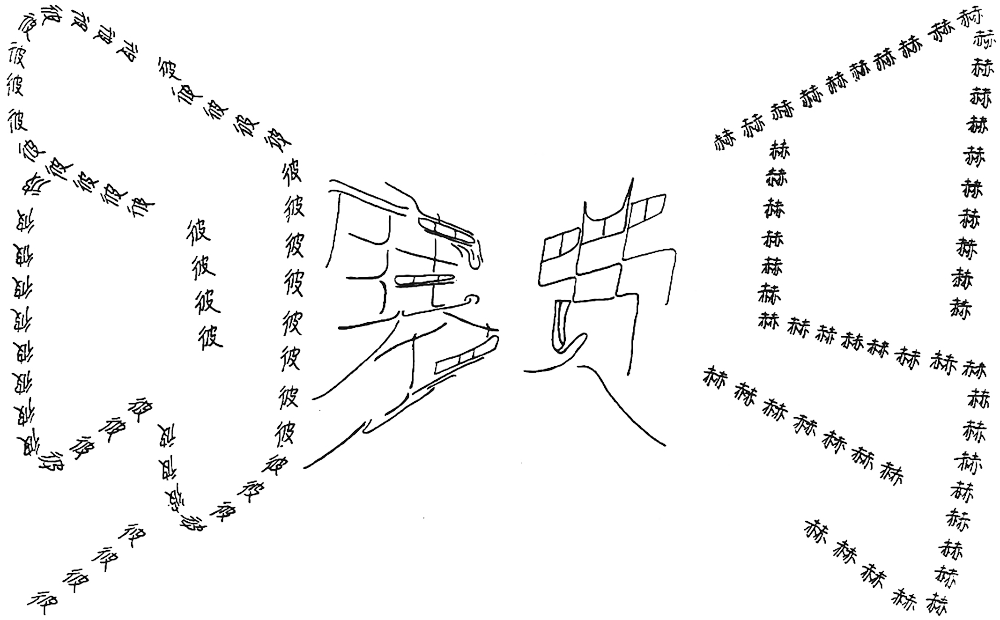
\includegraphics{img_062.png}
\caption[两个伟大名字的“交织”。]
  {刘皓明绘。}
\end{figure}

\item[乌龟]在我浏览《平均律钢琴曲集》的这个可爱版本的时候,现在刚好翻过这页,我发现那两个延长记号中的一个马上就要出现了——你好好听听吧,阿基。

\item[阿基里斯]我会的,我会的。

\item[乌龟]对着这一页的地方还有一张古怪透顶的图。

\item[螃蟹]难道又有一张?

\item[乌龟]自己找吧。\dlnote{(把总谱递给螃蟹。)}

\item[螃蟹]啊哈!是四组小字。让我看看——分别是“彼”、“德”、“巴”、“赫”,各自出现了许多次。我纳闷,为什么中间的字大,两边的字小?

\item[食蚁兽]能让我看看吗?

\item[螃蟹]当然。

\item[食蚁兽]我看你是只见树木,不见森林了。实际上,这是四个大字:“约”、“塞”、“费”、“马”,中间的字小,两边的字大。阿基里斯,你看呢?

\item[阿基里斯]让我瞧瞧。嗯,我看这些字是越往右边越小。

\item[乌龟]它们能组成有意义的词吗?

\item[阿基里斯]嗯……“约”、“塞”、“巴”、“赫”。哦,我明白了。这是巴赫的姓名!

\item[乌龟]你这种看法真怪。我看这些字是越往右边越大,而且……组成了……一个人……的……姓……名,\dlnote{(他逐渐变慢,最后几个字拉得特别长。然后是一阵短暂的静默。突然,他又正常起来,好像什么都没有发生过似的。)}——“彼·德·费马”。

\item[阿基里斯]哦,我敢肯定你满脑子里都是数学家费马。你看什么都是费马最后定理。

\item[食蚁兽]你刚才说的对,龟兄——我在这首赋格里刚听到一个迷人的小段延长记号。

\item[螃蟹]我也听到了。

\item[阿基里斯]你们是说除了我人人都听到了?我开始觉得我有点笨了。

\item[乌龟]哎哎,阿基——别沮丧。我敢肯定你不会错过赋格的最后延长记号——马上就会出现的。不过,让我们回到刚才的题目上来吧,食大夫,你提到的那个有关马姨庄园的前所有者的伤感故事是怎么回事?

\item[食蚁兽]那位前所有者是位出类拔萃的人物,是有史以来最富于创造性的蚁群之一。他的名字叫蚁翰·塞巴斯蚁安·蜚蚂,一位专业数学家、业余音乐家。

\item[阿基里斯]他可真是多才多艺啊!

\item[食蚁兽]在他的创造力的颠峰期,他惨遭最不是时候的猝死。一天,那是夏天里非常炎热的一天,他外出想去避避暑,正好赶上一场疾风暴雨——是那种一百年左右才会有一次的大暴雨——真叫是从天而降,把蚁·塞·蜚蚂淋了一个落汤蚂蚁。因为这场暴雨突如其来没有任何预兆,蚂蚁们完全晕头转向了。几十年建立起来的如此完美的复杂机体瞬间便毁于一旦。真是个悲剧。

\item[阿基里斯]你是说所有的蚂蚁全都淹死了,这当然就是说可怜的蚁·塞·蜚蚂完蛋了?

\item[食蚁兽]实际上并没有。蚂蚁们打算重新振兴,它们中幸存的每只蚂蚁都爬到飘浮在激流洪涛上的各种树枝木棍上。可是在洪水消退、蚂蚁们重新回到它们巢穴附近的地面上时,整个组织已不复存在了。种姓分布已经彻底毁坏了,这些蚂蚁已无力重建曾经有过的那个协调得如此完美的组织。它们就像破碎的镜子一样不能指望重圆了。我就像所有的媒婆月老一样,企图把可怜的蜚蚂重新撮合到一块儿。我满怀信心地放了些糖和奶酪,徒劳地希望蜚蚂也许会重新合成……\dlnote{(掏出一块手帕擦他的眼睛。)}

\item[阿基里斯]你真英勇!我以前以不知道食蚁兽们竟有这么一副慈悲心肠。

\item[食蚁兽]不过这根本无济于事。他去了,不可能再重建。可是随后发生了一件非常奇怪的事:在接下来的几个月里,那些过去是蚁·塞·蜚蚂成员的蚂蚁们慢慢儿又重新组合起来,并且建立了一个新的组织。因此马姨就诞生了。

\item[螃蟹]真了不起!马姨就是由组成蜚蚂的那些蚂蚁构成的?

\item[食蚁兽]对,最初是这样的,没错儿。而现在,有些老蚂蚁已经死掉了,被替代了。但是有一些从蚁·塞·蜚蚂时代留下来的遗老还活着。

\item[螃蟹]你偶尔也会在马姨身上找到某些明显的蚁·塞·蜚蚂的旧特征吗?

\item[食蚁兽]一点也找不到。他们毫无共同之处。而且在我看来,也没有任何理由应该这样。重新组织许多部分以构成一个“总和”,毕竟有着许多种彼此不同的方式。而马姨只不过是旧的各部分的一种新“总和”而已。注意,并没有多于那个总和——只是这个特定种类的总和。

\item[乌龟]说到总和,叫我想起了数论。在数论里有时可以把一个定理拆卸成它的各构成符号,再以一种新的顺序重新组织它们,从而得出一个新定理。

\item[食蚁兽]我从未听说过这种现象。不过我承认在这一领域里我完全是个外行。

\item[阿基里斯]我也没听说过——而我对这一学科是颇为精通的,也许我自己不该这么说。我怀疑龟兄不过是在打哈哈。如今我可太了解他了。

\item[食蚁兽]说到数论,又叫我想起了蚁·塞·蜚蚂,因为数论是他拿手的领域之一。事实上,他对数论作出过某些十分了不起的贡献。而马姨则在任何哪怕跟数学沾一丁点儿边的事情上都极其迟钝。此外,她在音乐方面的趣味不过平平而已,而塞巴斯蚁安在音乐方面极有天才。

\item[阿基里斯]我非常喜欢数论。你能不能给我们讲一讲塞巴斯蚁安做出的那些贡献的本质?

\begin{figure}
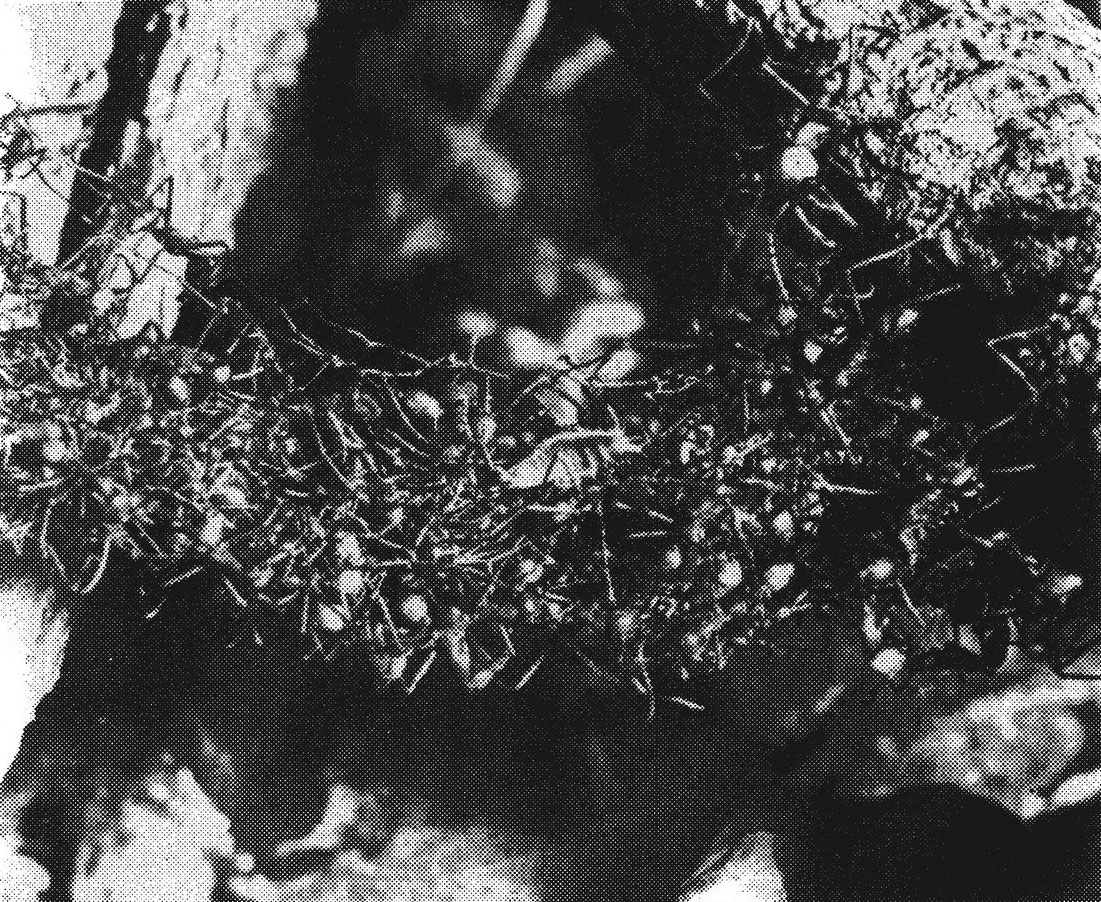
\includegraphics{img_063.jpg}
\caption[一座蚁桥的照片。]
  {徙途中,兵蚁有时会用它们自己的身体搭起一座活桥。在这幅照片中就是这样一座桥。可以看到一个蚁群的工蚁们腿脚相连,它们的跗节肢钩在一起,顺着桥头形成许多不规则的链系统,一只共生的蠢鱼正在过桥,此时它处在中心部位。引自爱德华·威尔逊的《昆虫社会》!}
\end{figure}

\item[食蚁兽]好吧。\dlnote{(停顿了一小会儿,呷了一口茶,然后才开始说起来。)}你们听说过狒犸那个臭名昭著的“平均验刚劲猜想”吗?

\item[阿基里斯]我说不好……听起来怪熟的,可我想不起来了。

\item[食蚁兽]内容非常简单。溺爱儿·的·狒犸,这位专业数学家、业余律师,在读一本丢饭蠹的经典教本《算术》时,看到了这样一个方程式:
\[
  2^a+2^b=2^c
\]
他立刻意识到有无穷多个$a$、$b$、$c$能满足这个方程,于是在书的边空上写下了下面这段臭名昭著的批注:
\begin{quote}
方程
\[
  n^a+n^b=n^c
\]
其中$a$、$b$、$c$及$n$取正整数,仅当$n=2$时有解(此时将有无穷多的三元组$a$、$b$、$c$满足这个方程);但$n>2$时没有解。我已找到了一个精彩的证明,可是不凑巧,这个证明太小了,如果写在这块边空上几乎会看不清。
\end{quote}
从三百多天前的那年起,数学家们绞尽脑汁,试图做到:或者证明狒犸的断言,从而维护狒犸的声誉——因为由于一些人怀疑他并没有真的找到他所说的那个证明,狒犸的名声多少有些不佳了——或者否定狒犸的断言,找出一个反例:给出四个整数$a$、$b$、$c$和$n$,其中$n>2$,满足那个方程。直到最近,这两个方向上的努力都是失败的。诚然,这个猜想已经在许多具体的$n$值上被验证是成立的——即那些小于$12500$的$n$值。但是没有人成功地证明它对所有的$n$值都成立——没有人,这就是说,直到蚁翰·塞巴斯蚁安·蜚蚂出现之前。是他发现了那个证明,从而保住了狒犸的名誉。现在它的名字是“蚁翰·塞巴斯蚁安的平均验刚劲猜想”。

\item[阿基里斯]如果正确的证明最终给出了,是不是应该把它称作“定理”而非“猜想”?

\item[食蚁兽]严格说来,你是对的,但习惯上一直这么叫。

\item[乌龟]塞巴斯蚁安写了些什么样的音乐?

\item[食蚁兽]他在作曲方面极有天赋。不幸的是,他的最伟大的作品被罩在一层神秘的网下,因为他从未发表过它。有人确信那整部作品都在他的心里,另一些人则不太客气,说他也许压根儿就没有作过这支曲子,只不过是吹吹牛而已。

\item[阿基里斯]这部巨作是什么性质的?

\item[食蚁兽]是一部庞大的前奏曲和赋格,其赋格将有二十四个声部,涉及二十四个不同的主题,每一主题各有一个大调和一个小调。

\item[阿基里斯]把二十四个声部的赋格作为一个整体来听一定很难!

\item[螃蟹]更别说创作这么一部曲子了!

\item[食蚁兽]但是我们所知道的有关它的一切就是塞巴斯蚁安对它的描述,他把这段描述写在了他的那本为管风琴而写的幂幂地加在一起的前奏曲和赋格曲的空白处。在他悲剧性的猝亡前,他写的最后几句话是:
\begin{quote}
我已写成了一部精彩的赋格。在里面我将调的$24$次幂与主题的$24$次幂加了起来,作出了一部具有$24$个声部幂的赋格。可是不凑巧,这里的边空太小了,我无法写下它。
\end{quote}
这部未能实现的杰作就被命名为《蜚蚂的最后赋格》。

\item[阿基里斯]哦,这真是个叫人受不了的悲剧。

\item[乌龟]说起赋格,我们一直在听的这支赋格就要结束了。在接近结尾的时候,主题会出现一个奇怪的新转折。\dlnote{(翻阅《平均律钢琴曲集》)}哎,这是什么?又是一幅插图——多吸引人呀!\dlnote{(给螃蟹看。)}

\item[螃蟹]哎,这是什么?哦,我明白了:是“整化论”,是用大个儿字写的,先是缩小,然后又恢复到原来的尺寸。可这毫无意义,因为这不是一个词。嘿,怎么搞的,嘿,真是的!\dlnote{(把它递给食蚁兽。)}

\item[食蚁兽]哎,这是什么?哦,我明白了:是“简体论”,是用小个儿字写的,先是变大,然后又缩小到原来的尺寸。可这毫无意义,因为这不是一个词。嘿,真是的,嘿,怎么搞的?\dlnote{(把它递给阿基里斯。)}

\item[阿基里斯]我知道你们大家肯定不会相信:可事实上这幅图是由“整体论”一词组成的,方块儿字从左向右不断缩小,“体”字是草体,所以老蟹认错了。\dlnote{(把它还给了乌龟。)}

\begin{figure}
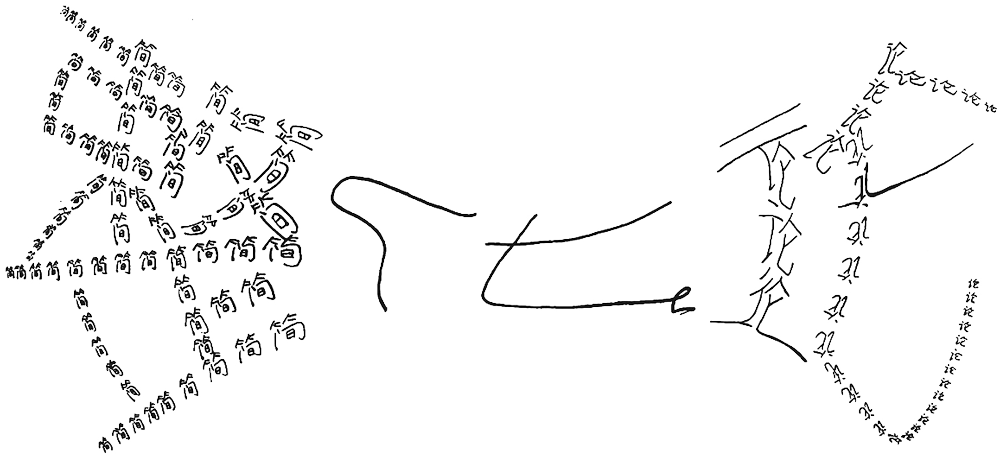
\includegraphics{img_064.png}
\caption[一支整体论—简化论的“螺旋桨”。]
  {刘皓明绘。}
\end{figure}

\item[乌龟]我知道你们大家肯定不会相信,可事实上这幅图是由“简化论”一词组成的,方块儿字从左向右不断增大。“化”字是草体,所以食大夫认错了。

\item[阿基里斯]这次我终于听到主题的那个新转折了!真感谢你给我的指点,龟兄。我想我最终还是开始掌握听赋格的艺术了。

\end{dialogue}

\end{dialog}
